%!TEX root = thesis.tex

\chapter{Related Work}
\label{ch:relatedwork}

In this section, previous research regarding the topic of battles on Pokémon Showdown is described and compared.

\section{Baseline Agents}
\label{sec:eval-challenges-baseline}
A good way to get a rough idea on how well an agent performs is to compare it against a baseline agent.
There are two popular baseline agents, the \textit{Random}-Player and the \textit{MaxDamage}-Player.
While the \textit{Random}-Agent always chooses either a random move or a random switch, the \textit{MaxDamage}-Agent
always picks the move with the highest base power. If no move is available, the agent will switch to a random 
Pokémon. This is roughly equal to the skill level of an inexperienced beginner human. 

\section{Breadth-first search}
\label{sec:related-bfs}
Given a root battle object representing the current game state, \ac{BFS} explores the outcomes of all possible choices,
treating these resultant states as child nodes. This algorithm traverses the game tree until it finds a state in which
the enemy Pokémon is fainted. As a non-adversarial algorithm, the agent assumes that the agent does not move at all.
This agent won 75 out of 90 total games played against a random agent~\autocite{Lee_Togelius_2017}.

\section{Minimax}
\label{sec:related-minimax}
Minimax builds upon \ac{BFS} as this algorithm deals with adversarial paradigms by assuming the opponents 
act in their best interest.
There are multiple possibilities on how to implement the Minimax algorithm for Pokémon games. The main difference 
in implementations lies in state evaluation and the assumptions about the opponents. Additionally,
the amount of features taken into consideration have a considerable impact. In the implementation proposed by
\cite{Lee_Togelius_2017}, a node represents the worst case scenario that would occur as a result of the current choice. 
The agent also employes alpha-beta pruning, ignoring any node in which the agents Pokémon faints. 
One drawback of this procedure is that, a Pokémon would never use the move \textit{Explosion},
a very powerful \textit{Normal}-type move that also faints the user. This move can for example be used if
the active member is already at very low \ac{HP}.
The tree itself is traversed using a greedy strategy, which terminates when a state in which the enemy 
Pokémon is fainted is reached. Both the traversal order and the worst-case evaluation are performed using
the evaluation function \ref{eq:minmax-eval-func}~\autocite{Lee_Togelius_2017}:
\begin{equation}
\label{eq:minmax-eval-func}
    Eval = \frac{\text{current hp}_{\text{Own Pokémon}}}{\text{max hp}_{\text{Own Pokémon}}} -
    3 \cdot \frac{\text{current hp}_{\text{Enemy Pokémon}}}{\text{max hp}_{\text{Enemy Pokémon}}} -
    0.3 \cdot \text{depth}
\end{equation}
A YouTube-Video released by \emph{Rempton Games} \cite{RemptonGames:PokemonAI} \todo{This quote is even stranger} 
alters this evaluation function
by increasing the rating of a game state when an enemy takes damage and decreasing the rating when a member
of the own team takes damage. Both evaluation functions do not take hazards, status condition or boosts 
into account. Due to the similarity of both evaluation functions, both agents performed very similarly:
The first agent described by \cite{Lee_Togelius_2017} won 70 out of 90 total games against a random agent,
resulting in a win-ratio of $\approx 86\%$. The second agent defeated the random player in 831 out of 1000
total games, yielding a win-ratio of $\approx 83\%$. Due to the large amount of \ac{RNG} in battles, we assume
both agents to be at an equal level of play. \\
The current state of the art search-based algorithm was developed by \emph{pmariglia} and is fully available
at \cite{Github:pmariglia-showdown}. This approach uses the \textit{Expectiminimax}-Algorithm and takes
hazards, boosts and status into consideration. In addition to \grqq min\grqq{}
and \grqq max\grqq{} nodes of a traditional \emph{Minimax}-tree, this variant has \grqq chance\grqq{} nodes, which take the 
expected value of a random event occurring~\autocite{wiki:Expectiminimax}. Currently, the agent calculates two turns in
advance, and reaches an Elo rating of $1461$ as well as a Glicko-1 rating of $1633$ in Generation VII random battles 
on the Showdown ladder. 
In addition, \emph{pmariglia} implemented an algorithm to estimate the item a Pokémon is holding
based on the damage it dealt. 

\section{Rule based agents}
\label{sec:related-rulebased}
The YouTube-Video released by \emph{Rempton Games} \cite{RemptonGames:PokemonAI} also introduces two rule-based agents.
\textit{Smart Damage} was written by the author of the video and uses Pokémon type and the \ac{SPE}-stat to determine
the favorability of a matchup. On a bad matchup, this agent will switch to the team member with the best matchup. Otherwise,
a simplified damage calculation is used to determine the move dealing the most amount of damage. \textit{Simple 
Heuristics} was developed by, \emph{Haris Sahovic}, the author of the \emph{Poke-Env} library \cite{PokeEnv:Github}.
The implementation for this agent can be found at \cite{PokeEnv:Baselines}. This agent uses simple rules
to decide the next move or switch and takes boosts as well as hazards into account. The results for both agents
are denoted in table \ref{tbl:Youtube-Results}. The \emph{MiniMax}-agent in the table reffers to the implementation
of \emph{Rempton Games}.
\begin{table}[h]
    \centering
        \begin{tabular}{|l|l|l|l|l|l|}
            \hline
            & \emph{Random} & \emph{Max \ac{DMG}} & \emph{Smart \ac{DMG}} & \emph{Minimax} & \emph{Heuristics} \\
            \hline
            \emph{Random} & N / A & 897 / 103 & 957 / 43 & 831 / 169 & 992 / 8 \\
            \hline
            \emph{Max \ac{DMG}} & & N / A & 829 / 171 & 834 / 166 & 955 / 45 \\
            \hline
            \emph{Smart \ac{DMG}} & & & N / A & 331 / 669 & 720 / 280 \\
            \hline
            \emph{Minimax} & & & & N / A & 181 / 819 \\
            \hline 
        \end{tabular}
        \caption{Denotes how many games the Agent in the column won against the agent in the row \cite{RemptonGames:PokemonAI}}
        \label{tbl:Youtube-Results}
\end{table}

\section{Other approaches}
The authors of the \textit{Showdown AI Competition}~\autocite{Lee_Togelius_2017} compared many
simple AI implementations with each other. Approaches not covered so far will be summarized
in this chapter.


\paragraph{One Turn Lookahead}
\emph{One Turn Lookahead} is a heuristic agent designed to encapsulate a greedy strategy that 
prioritizes the damage output. The agent operates by estimating the damage dealt by all usable moves, 
including those usable by the agent's inactive but usable Pokémon. If the highest damaging move 
belongs to the active Pokémon, the agent will use that attack. If the most damaging move belongs to 
an inactive Pokémon, the agent will switch to that Pokémon~\autocite{Lee_Togelius_2017}. Depending 
on implementation details, this agent is very similar to \emph{MaxDamage} or \emph{Rule based}
agents.

\paragraph{Type Selector}
This is a variation of the \textit{One Turn Lookahead}-Agent that utilizes a short series of
if-else statements in its decision-making. At first, if the current Pokémon knows a move 
that drains the opponents \ac{HP} to zero, this move is selected. Otherwise, the 
favorability of the current matchup is evaluated. If the current type matchup is 
undesirable, the agent will switch to the Pokémon with an acceptable type matchup. If no
such Pokémon exists, the agent will default to the most damaging move~\autocite{Lee_Togelius_2017}.

\paragraph{Pruned Breadth-First Search}
This agent is designed to demonstrate a simple way to utilize domain knowledge as a cost-cutting 
measure. This is achieved by making modifications to the Breadth First Search agent. First, 
the algorithm does not simulate any actions that involve using a damaging move with a resisted type, 
nor does it simulate any actions that involve switching to a Pokémon with a subpar type matchup. 
Additionally, rather than selfishly assuming the opponent skips their turn in each simulation, the 
agent assumes its opponent is a \emph{One Turn Lookahead}-agent and simulates 
accordingly~\autocite{Lee_Togelius_2017}.

\paragraph{Results}
Table \ref{tbl:AI-Comp-Results} displays the results of the agents described in this section.
\begin{table}[h]
    \centering
        \begin{tabular}{|l|l|}
            \hline
            & \emph{Random} \\
            \hline
            \emph{One Turn Lookahead} & 77 / 90 \\
            \hline
            \emph{Type Selector} & 67 / 90 \\
            \hline
            \emph{Pruned \ac{BFS}} & 75 / 90 \\
            \hline
        \end{tabular}
        \caption{Results of other approaches against a random agent~\autocite{Lee_Togelius_2017}}
        \label{tbl:AI-Comp-Results}
\end{table}

\section{Self-Play Policy Optimization Approach}
Researchers from \textit{New York University}~\autocite{Lee_Togelius_2017} were the first ones to apply
\textit{Q-Learning} to the field of Pokémon battles. Two agents using \textit{Q-Learning}
were developed: A single layer perceptron as well as a multi layer perceptron. Both agents were 
used to output the expected reward of all current moves and switches. Based on this, the best 
action was picked. Both agents were rewarded for defeating opponent Pokémon and punished for 
allowing one of its own Pokémon to faint. Because decisions made tend to have long term consequences, 
weights are updated using the last three (State, Action) pairs rather than the most recent pair only.
Additionally, in order to promote exploration, the agent employs an epsilon-greedy selection policy, 
causing it to randomly override its decision with a probability of 0.1. The single layer perceptron 
was trained using the Delta Rule, while the multilayer perceptron was trained using Delta Rule 
plus Backpropagation. The agent using a single layer perceptron won $90$ out of $180$ games against a
random agent whereas the multi layer perceptron won 86 out of $180$ games. Due to the large amount
of \ac{RNG} in Pokémon games, more games would need to be played in order to confirm the superiority
of the single layer perceptron in this particular use case. Randomness of games will be covered
in more detail in section \ref{sec:eval-challenges-randomness}\\

One year after the publication of \cite{Lee_Togelius_2017}, the authors of 
\todo{Include GottaTrainEmAll in BIB!! (Zotero)}
\cite{GottaTrainEmAll} 
improved this design. \cite{schulman2017proximal} used \ac{PPO} to train an agent. They also
used embeddings to improve the representation of a Pokémon. Data available at~\autocite{Kaggle:NewYorkData} was used
to create embeddings for each Pokémon. The Dataset contains stats of the first 721 Pokémon, each 
row contains the name, type(s), numerical stat data (such as \ac{HP}, \ac{ATK}, \ac{SPE}) and some other
data such as color, height and whether the Pokémon is considered legendary in game. To create
embeddings for each Pokémon, the data was turned into a graph to be used with Node2Vec~\autocite{grover2016node2vec} 
which creates embeddings from graph data in similar to
Word2Vec~\autocite{mikolov2013distributed}. This algorithm samples random walks of some number
of nodes of a given graph. Using these random walks, a skip-gram model is created which
can be trained to generate embeddings. The Pokémon graph consisted of the name, type(s),
numerical attributes (total stats, \ac{HP}, \ac{ATK}, \ac{DEF}, \ac{SPA}, \ac{SPD}, \ac{SPE})
as well as two special nodes, \textit{Legendary} and \textit{Mega}\footnote{Mega 
is a mechanic similar to dynamaxing. Mega is not available in the latest version of the game
and therefore won't be covered in detail}.
Lastly, Node2Vec was applied to the graph.
\begin{table}[h]
    \centering
        \begin{tabular}{|l|p{0.7\textwidth}|}
            \hline
            Pokémon & Most similar Pokémon \\
            \hline
            \emph{Bulbasaur} & Chikorita, Turtwig, Nuzleaf, Petilil, Exeggucte, Skiploom, Jumpluff, Oddish, Budew \\
            \hline
            \emph{Caterpie} & Wurmple, Weedle, Kakuna, Metapod, Paras, Ledyba, Spinarak, Venonat, Silcoon \\
            \hline
            \tikz[baseline=(X.base)]\node [draw=red,fill=white!20,thick,rectangle,inner sep=3pt, rounded corners=4pt] (X) {Mewtwo}; 
                & Lugia, Mesprit, Mew, Victini, Celebi, Cresselia, Volcation, 
                \tikz[baseline=(X.base)]\node [draw=red,fill=white!20,thick,rectangle,inner sep=3pt, rounded corners=4pt] (X) {Ho-Oh};, 
                Uxie \\
            \hline
        \end{tabular}
        \caption{Similar Pokémon within the embedding space of \cite{GottaTrainEmAll}}
        \label{tbl:Gotta-Embeddings}
\end{table}
Table \ref{tbl:Gotta-Embeddings} displays the discovered similarity using this approach. Here, a similar Pokémon
to \textit{Mewtwo}, a \textit{Psychic}-Type, is \textit{Ho-Oh}, a \textit{Flying}-\textit{Fire}-Type. However,
these two have entirely different strengths and weaknesses. In addition to that, they do not share a single
move in their move set: 
In generation 6, \textit{Ho-Oh} has access to the following moves: \textit{Aura Sphere}, \textit{Calm Mind}, 
\textit{Fire Blast}, \textit{Ice Beam}, \textit{Psystrike} and \textit{Recover} whereas \textit{Lugia}'s
move pool consists of \textit{Brave Bird}, \textit{Earthquake}, \textit{Flame Charge}, \textit{Roost},
\textit{Sacred Fire}, \textit{Substitute} and \textit{Toxic}~\autocite{DamageCalc:Gen6}. This inappropriate
classification is likely caused by both \textit{Pokémon} having similar stats and both being legendary.
\todo{The paper states that they are confident in their embeddings. This critic is my own work. How
do I note this properly?}

Features are derived from the battle state in the simulator. At a high level, battles consist of two
sides. Each side consists of a team of Pokémon, and each Pokémon has some set of moves. Each of these 
objects (battle, side Pokémon, and move) have attributes that are used to derive a feature vector.
After experimenting with multiple network architectures, the authors settled on a three-layer 
fully connected neural network, each with 512 neurons and a ReLU activation function.

The authors of~\cite{GottaTrainEmAll} trained the agent against a random agent, a default agent 
that always tries to pick a non-switching move as well as a \emph{Minimax}\footnote{The Authors don't
provide implementation details of their \emph{Minimax} implementation} agent
until the reward curve stabilized which was around 100 epochs where an epoch is a single battle between
two players. A reward of $+1$ is given to the agent if it wins the battle, $-1$ if it loses the battle and
$0$ for all other cases. The average epoch reward after training convergence for this approach can
be found in table \ref{tbl:Gotta-Performance}
\begin{table}[h]
    \centering
        \begin{tabular}{|l|l|}
            \hline
            Opponent & Average epoch reward \\
            \hline
            \emph{Random} & $0.85$ \\
            \hline
            \emph{Default} & $0.85$ \\
            \hline
            \emph{Minmax} & $-0.9$ \\
            \hline
        \end{tabular}
        \caption{Average epoch rewards after training convergence for opponent agents~\autocite{GottaTrainEmAll}. Agent
        outperforms random and default agent but fails to defeat the Minimax-agent.}
        \label{tbl:Gotta-Performance}
\end{table}
The authors of \cite{GottaTrainEmAll} describe their final agent as flawed as while the agent learned 
to switch Pokémon when the active Pokémon reaches low health, it almost always chooses to switch to the
Pokémon in the last slot. In addition, this agent preferentially chooses the fourth move. 

\subsection{State of the art}
In 2019, \cite{Huang_Lee_2019} published a paper titled \emph{A Self-Play Policy 
Optimization Approach to Battling Pokémon}. 
Due to its fine-grained analysis and the resulting agent performing on par with the state-of-the-art search
based AI, this paper will be summarized in more depth. \\
Similar to \cite{OpenAI_dota}, the agent is represented using an actor-critic neural network.
Actor-critic RL methods~\autocite{Konda_Tsitsiklis}\todo{Citation broken}
combine policy-based and value-based RL methods by predicting both policy and value for a given 
state, and then using the value prediction, the \grqq critic\grqq, as an estimate of expected
return when updating the policy prediction, the \grqq actor\grqq. The authors represent both
actor and critic using a two-headed neural network which is trained via self-play RL~\autocite{Huang_Lee_2019}.

\paragraph{Neural Network}
Input to the neural network is the current state of the game, from the point of view of the player,
represented as multi-level tree-like structure:
\begin{enumerate}
    \item The \textit{battle} consists of two \textit{teams}, along with weather effects.
    \item Each \textit{team} consists of six \textit{Pokémon}, along with side conditions 
    described in section \ref{sec:field-effects}
    \item Each \textit{Pokémon} has many features. Table \ref{tbl:HuangLee-Pokemon-Table} contains a partial 
    list\footnote{The authors state that this list is not complete, but no additional information is provided.}
\end{enumerate}
\begin{table}[h]
\centering
    \begin{tabular}{llll}
    \hline \\
    Feature             & Type        & Dims            & Description                 \\
    \hline \\
    \emph{species}      & categorical & $1 \times 1023$ & e.g. Pikachu                \\
    \emph{item}         & categorical & $1 \times 368$  & e.g. Leftovers, Choice Band  \\
    \emph{ability}      & categorical & $4 \times 238$  & e.g. Rough Skin, Shadow Tag \\
    \emph{moveset}      & categorical & $4 \times 731$  & e.g. Flamethrower, Surf     \\
    \emph{lastmove}     & categorical & $1 \times 731$  & The last move used          \\
    \emph{stats}        & continuous  & 6               & \ac{HP}, \ac{ATK}, \ac{DEF}, \ac{SPA}, \ac{SPD}, \ac{SPE} \\
    \emph{boosts}       & continuous  & 6               & Temporary boosts for stats \\
    \emph{hp}           & continuous  & 1               & Current number of \ac{HP} \\
    \emph{maxhp}        & continuous  & 1               & Number of \ac{HP} at full health \\
    \emph{ppUsed}       & continuous  & 4               & \# times a move was used \\
    \emph{active}       & indicator   & 1               & 1 if Pokémon is active, else 0 \\
    \emph{fainted}      & indicator   & 1               & 1 if Pokémon has no \ac{HP}, else 0 \\
    \emph{status}       & indicator   & 28              & e.g. \ac{SLP}, \ac{BRN}, \ac{PAR} \\
    \emph{types}        & indicator   & 18              & e.g. \textit{Bug}, \textit{Fire} \\
    \emph{volatiles}    & indicator   & 23              & e.g. Leech Seed, Perish Song
    \end{tabular}
    \caption{Features used to describe a single Pokémon battle~\autocite{Huang_Lee_2019}}
    \label{tbl:HuangLee-Pokemon-Table}
\end{table}
The network has two outputs: a probability distribution $\pi \in \mathbb{R}^n$ over actions to take, 
and an estimate of player strength in the current state $v \in \mathbb{R}$. \cite{Huang_Lee_2019} compute
$\pi$ as follows:
\todo{Move neural network figure to the appendix}
\begin{enumerate}
    \item The network outputs an intermediate vector $p \in \mathbb{R}^n$. Each of the colored cells in
    figure \ref{fig:lee-network} correspond to an element of $p$
    \item A probability distribution $\pi' \in \mathbb{R}^n$ is computed by using the
    softmax function: \\ $\pi' = \frac{\exp(p_i)}{\sum_i \exp(p_i)}$
    \item As not every action is valid in every state, for example, a switch to a Pokémon is invalid
    if that Pokémon is already fainted, the authors ensure their agent has zero probability of taking
    invalid actions. To do this, they take a mask $s \in \{0, 1\}^n$ as part of the input, and 
    renormalize probabilities to obtain $\pi: \pi_i = \frac{s_i \pi'_i}{s^T \pi'}$
\end{enumerate}
\begin{figure}
	\centering
	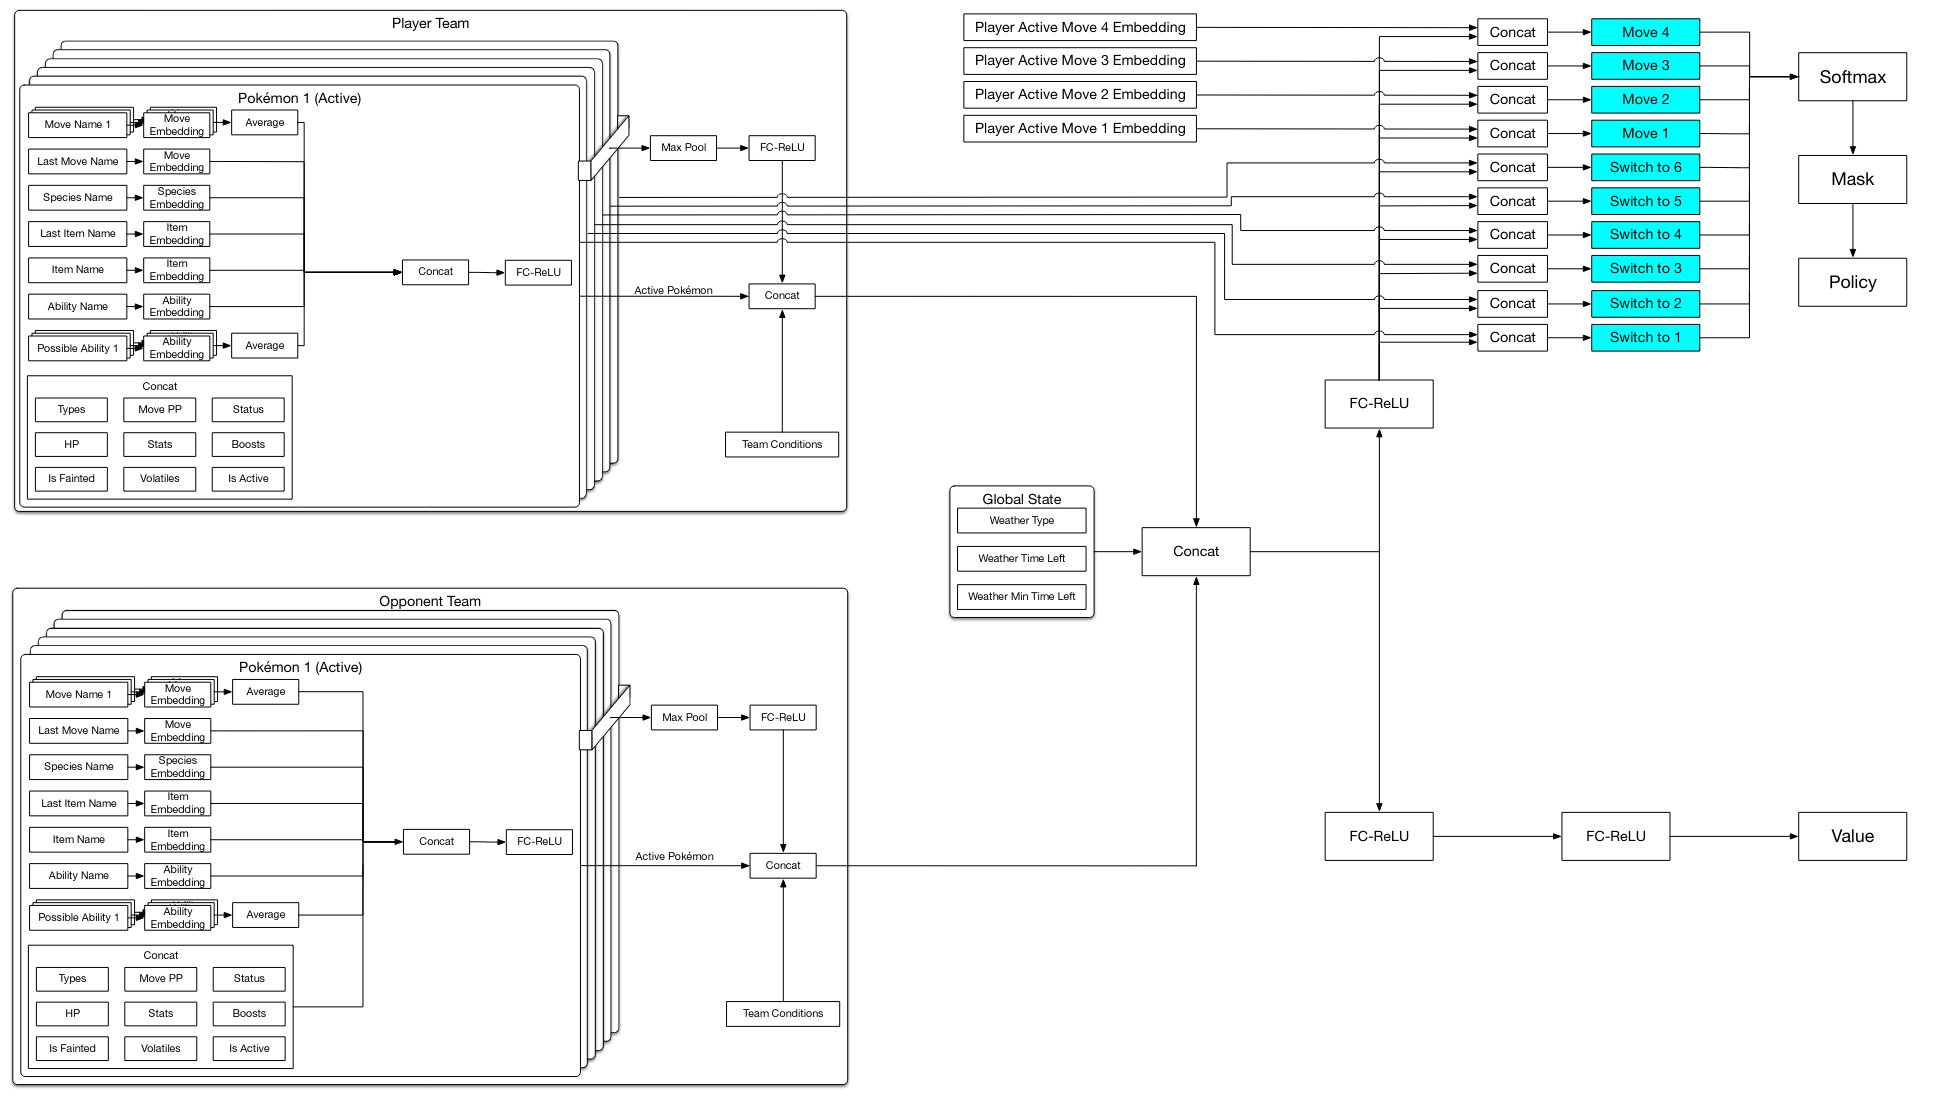
\includegraphics[width=1\textwidth]{images/RL-Network-Structure.png}
	\caption{The actor-critic neural network used by the authors in~\autocite{Huang_Lee_2019}}
	\label{fig:lee-network}
\end{figure}
The authors point out the following two key design decisions: First, a 128-dimensional entity embedding layer
for each of the categorical variables is used. This enables capturing similarities between different moves,
species and abilities without having to directly model their, often complicated, effects. Second, the
parameters for computing $p$ from above are shared among all $n$ actions. The resulting network is described
by figure \ref{fig:lee-network} and contains 1,327,618 parameters in total~\autocite{Huang_Lee_2019}.

\paragraph{Training the network}
Training was done serially: After $m = 7680$ games per iteration, the neural network parameters are updated
using the $2m$ self-play matches as training data to obtain new neural network parameters. A reward
of $+1$ for a win and $-1$ for a loss is assigned at the end of the match. To speed up learning, a 
dense reward signal using reward shaping was constructed. Auxiliary rewards are assigned based on
events that occur over the course of the match. For example, a reward of $-0.0125$ is added when a 
Pokémon of the agent faints, and a reward of $+0.0025$ whenever the player's Pokémon makes a 
super effective move\footnote{While the authors do not provide an exact definition, we assume
that a move is regarded as \textit{super effective}, if the type modifier described in 
\nameref{sec:damage-calculation} is bigger than one}. \\
To update the neural network, the authors use \textit{Proximal Policy Optimization}~\autocite{schulman2017proximal}, which optimizes
an objective function that combines expected reward, accuracy of state value prediction, and a bonus
for high entropy policies. To reduce the variance of policy gradient estimates, \textit{Generalized
Advantage Estimation}~\autocite{schulman2018highdimensional} is used. \\
After 500 iterations of the training loop, 3,840,000 self-play matches had been played by the neural
network. Training was performed using Google Cloud Platform over the course of 6 days with an 
approximated cost of \$91 USD.

\paragraph{Evaluation}
\label{sec:dqn-evaluation}
The refined embeddings as well as the complex network architecture lead to this agent outperforming
the RL-Agent described in \cite{GottaTrainEmAll}. Furthermore, the agent played 1.000 games against
the open source agent of \textit{pmariglia} mentioned in \ref{sec:related-minimax}
\begin{table}[h]
    \centering
        \begin{tabular}{|l|l|l|}
            \hline
            \textbf{Opponent} & \textbf{Wins} & \textbf{Losses} \\
            \hline
            \emph{random} & 995 & 5 \\
            \hline
            \emph{max-damage} & 929 & 71 \\
            \hline
            \emph{max-damage-typed} & 829 & 171 \\
            \hline
            \emph{pmariglia} & 612 & 388 \\
            \hline
        \end{tabular}
        \caption{Performance of the agent developed by \cite{Huang_Lee_2019}}
        \label{tbl:State-Of-The-Art-Results}
\end{table} 
Table \ref{tbl:State-Of-The-Art-Results} describes the performance of the agent developed by
\cite{Huang_Lee_2019}.
While the authors do not provide the resulting Elo oft the agent, they state that a 
\textit{Glicko-1} rating of 1677 was reached. It is important to note that this agent played
against an older version of \textit{pmariglia} which was released in May 2019. Results
of this agent described in section \ref{sec:related-minimax} and section \nameref{ch:evaluation} 
used the latest release as of February 2022.

\section{Supervised Approach}
As of writing, there is only one publication researching supervised learning for Pokémon battles,
a YouTube video uploaded to the channel \grqq\emph{The Third Build}\grqq{}~\cite{TheThirdBuild:PokemonAI}.
Unfortunately, the video does not cover much technical and implementation details, possibly to reach a 
broader audience on YouTube.
The author obtained two million 
replays of human games from the creators of Pokémon Showdown. Using these replays, the input vector for a game
contained the following features is created:
\begin{itemize}
    \item \textbf{Pokémon attributes:} \ac{HP}, whether the Pokémon is active, status condition and stat boosts.
    \item \textbf{Player's side attributes:} side conditions (like \textit{Light Screen}), entry hazards 
    (like \textit{Stealth Rocks}), volatile conditions like \textit{Leech Seed} and the last used move
    \item \textbf{Battlefield attributes:} weather, pseudo-weather\footnote{The video does not give an exact 
    definition of the word \textit{Pseudo-Weather}} and terrain
\end{itemize}
Using these features, a neural network using TensorFlow for JavaScript was then trained to predict the 
win chance of a given player at a given state of the game. This network was able to predict the winner
at a given state with an accuracy of 81\%. In addition to that, the model was able to predict the next
switch in with an accuracy of 86\%, the next move with a certainty of 93\% and whether the
player would switch with an accuracy of 88\%. Unfortunately, the author neither states the game type of
the replays nor the exact architecture and evaluation method of the model. \\
This model was then used to pick the best move in a given scenario which allowed the agent to play games
on the Pokémon Showdown ladder. Unlike other agents quoted in this thesis, this agent does not play
\emph{random} battles on Pokémon Showdown, but rather \emph{Gen 8 OU Singles}. \\
Furthermore, \textit{Inverse Damage Calculation} is introduced. As the exact item of 
enemies are unknown, the author predicts the given item of a Pokémon by comparing the damage dealt
of a move with the expected damage for the move modified by possible items. Despite no concrete 
implementation details given, we assume this approach to work similar to the implementation 
of \emph{pmariglia} described in \ref{sec:related-minimax}.
According to the video, this agent reached a maximum Elo of $1630$ which ranks the agent among the 
best $3.6\%$ of players.